\documentclass[12pt]{article}
\usepackage[utf8]{inputenc}
\usepackage[T1]{fontenc}
\usepackage{pdflscape} 
\usepackage{lmodern}
\usepackage[a4paper,bindingoffset=0.2in,%
            left=0.5in,right=0.5in,top=0.5in,bottom=1in,%
            footskip=.25in]{geometry}
\usepackage[colorlinks=true, linkcolor=Black, urlcolor=Blue]{hyperref}
\usepackage{graphicx}
\usepackage{subcaption}
\usepackage{listings}
\usepackage{color}
\usepackage[table]{xcolor}
\definecolor{lightgray}{gray}{0.9}

\definecolor{codegreen}{rgb}{0,0.6,0}
\definecolor{codegray}{rgb}{0.5,0.5,0.5}
\definecolor{codepurple}{rgb}{0.58,0,0.82}
\definecolor{backcolour}{rgb}{0.95,0.95,0.92}

\lstdefinestyle{mystyle}{
	backgroundcolor=\color{backcolour},   
	commentstyle=\color{codegreen},
	keywordstyle=\color{magenta},
	numberstyle=\tiny\color{codegray},
	stringstyle=\color{codepurple},
	basicstyle=\ttfamily\footnotesize,
	breakatwhitespace=false,         
	breaklines=true,                 
	captionpos=b,                    
	keepspaces=true,                 
	numbers=left,                    
	numbersep=5pt,                  
	showspaces=false,                
	showstringspaces=false,
	showtabs=false,                  
	tabsize=2
}


\begin{document}
\title{Projekt - Drzewa Decyzyjne I\\
\large Sebastian Michoń 136770, Marcin Zatorski 136834\\
\large grupe L5}
\date{\vspace{-10ex}}
\maketitle

\section{Metoda ogólna - dane dyskretne}
\begin{enumerate}
	\item Wpierw dataset jest wczytany do formatu dataframe biblioteki pandas. Usuwane są nazwiska pasażerów i ich nry id.
	
	\item Wiek pasażera jest transformowany zgodnie z wytycznymi (to dotyczy tylko obliczeń dla 1. części projektu).
	
	\item Drzewo jest tworzone jako tablica podzbiorów dataframe'a: na początku, w korzeniu drzewa (w 0. elemencie listy) dany jest cały dataframe; jeśli możliwy jest split w danym wierzchołku (i gain ratio wynikający z tego splita jest większy od 0), to dataframe w wierzchołku jest dzielony według kolumny, split na której daje najwyższy gain ratio. Każdy powstający podzbiór dataframe'a jest dodawany na koniec tablicy wierzchołków. Razem z nimi dla każdego wierzchołka uzyskuję informacje o nrze ojca i splicie, w wyniku którego powstał (który jest wygodny do późniejszego rysowania drzewa).
	
	\item Entropia, entropia warunkowa, gain ratio, information gain i intristic information są liczone jawnie ze wzoru - w ogólności złożoność obliczeniowa kalkulowania kolejnego splita to \(O(n\sum_{i=0}^{m}{x_i})\), gdzie \(n\) to liczba wierszy dataseta w danym wierzchołku, \(m\) to liczba atrybutów, a \(x_i\) to liczba różnych wartości w \(i\)-tym atrybucie dla dataframe'a w tym wierzchołku.
	
	\item W momencie, w którym nie da się uzyskać lepszego od 0 gain ratio w danym wierzchołku (może zajść, gdy żadna pojedyncza kolumna nie pozwala lepiej sklasyfikować zbioru danych niż sam wierzchołek), nie jest dokonywany żaden split (co nie oznacza, że nie byłoby zasadnym go dokonać - natomiast algorytm podziału jest zachłanny, więc działa w taki a nie inny sposób). Jeśli nie da się dokonać żadnego kolejnego splita konstrukcja drzewa się kończy. Przykład dataseta, w którym 2 splity prowadziłyby do wzrostu współczynnika informacji, choć żaden nie zostanie wykonany: (Y to atrybut, którego wartość chcemy poznać w zależności od c1, c2)\\
		\begin{tabular}{lll}
			c1 &  c2 &  Y \\
			A & B & 1 \\
			B & A & 1 \\
			A & A & 0 \\ 
			B & B & 0 \\ 
		\end{tabular}
	
	\item W ostatniej fazie rysowane jest drzewo - w osobnym pliku otwierającym się na poziomie jupytera, jako że wygodniej jest przeglądać duży obrazek właśnie w takiej formie niż jako standardowy obrazek wewnątrz jupytera; wierzchołek opisany jest w formacie "1:x / 0:y", który oznacza, że w wierzchołku jest x obserwacji mających w polu "Survived" wartość 1 i y obserwacji mających w polu "Survived" wartość 0. Na krawędzi pokazywany jest split który do powstania tego wierzchołka doprowadził.
\end{enumerate}

\section{Metoda dla danych ciągłych}
\begin{enumerate}
	\item Dla danych ciągłych split na atrybucie C dzieli zbiór obserwacji na 2 części: Obserwacje z wartością \(x\) atrybutu C: \(x \le f\) i obserwacje z wartością \(x\) atrybutu C: \(x > f\) dla \(f\) nazywanego dalej miejscem splita.
	\item Miejsce splita jest wybierane jako takie miejsce, podział w którym maksymalizuje gain ratio. Proba znalezienia gain ratio opisanym powyżej (dla danych dyskretnych) algorytmem działałaby w złożoności \(O(n^2)\) dla \(n\) będącego liczbą wierszy dataseta, co jest niestaysfakcjonujące.
	\item Można także posortować dataset po atrybucie C, przesuwać potencjalne \(f\) do przodu, modyfikując dynamicznie listy wartości do obliczania warunkowej entropii i intristic info w czasie stałym i kalkulować je także w czasie stałym - złożoność zatem wyniesie \(O(nlog(n))\)
\end{enumerate}

\section{Działanie algorytmu - Logi (wersja na 5.0)}
W kolejnych wierszach: pokaz przebiegu algorytmu (jako logi) dla kilku pierwszych wierzchołków dla przypadku z ciągłym atrybutem Age.
\begin{verbatim}
	New vertex is processed: this vertex contains
	- 40 survived observations
	- 60 deceased observations
	The splits that led to the advent of this vertex were:
	[]
	Now, the possibility of split on attribute Pclass is processed
	Calculated entropy for "Survived" attribute is equal to 0.970951
	Calculated conditional entropy after splitting dataset on column Pclass
	Calculated conditional entropy is equal to 0.889278
	Information gain info is equal to:
	entropy-conditional_entropy=0.970951-0.889278=0.081672
	Intristic info is equal to 1.370229
	Gain ratio for discrete attribute C is calculated as:
	information_gain(C, Y)/intristic_info(C)=0.081672/1.370229=0.059605
	column: Pclass, gain ratio: 0.059605, attribute discrete
	
	Now, the possibility of split on attribute Sex is processed
	Calculated entropy for "Survived" attribute is equal to 0.970951
	Calculated conditional entropy after splitting dataset on column Sex
	Calculated conditional entropy is equal to 0.579428
	Information gain info is equal to:
	entropy-conditional_entropy=0.970951-0.579428=0.391523
	Intristic info is equal to 0.970951
	Gain ratio for discrete attribute C is calculated as:
	information_gain(C, Y)/intristic_info(C)=0.391523/0.970951=0.403236
	column: Sex, gain ratio: 0.403236, attribute discrete
	
	Now, the possibility of split on attribute Age is processed
	Solution is shown only for best possible split on this column, as
	otherwise it would be too long
	Calculated entropy for "Survived" attribute is equal to 0.970951
	Intristic info is equal to 0.080793
	Calculated conditional entropy after splitting dataset on column Age on x<=1
	Calculated conditional entropy is equal to 0.957622
	Information gain info is equal to:
	entropy-conditional_entropy=0.970951-0.957622=0.013329
	Gain ratio for continuous attribute C is calculated as:
	information_gain(C, Y)/intristic_info(C)=0.013329/0.080793=0.164974
	column: Age, gain ratio: 0.164974, split value: 1
	
	Now, the possibility of split on attribute SibSp is processed
	Calculated entropy for "Survived" attribute is equal to 0.970951
	Calculated conditional entropy after splitting dataset on column SibSp
	Calculated conditional entropy is equal to 0.930295
	Information gain info is equal to:
	entropy-conditional_entropy=0.970951-0.930295=0.040655
	Intristic info is equal to 1.619082
	Gain ratio for discrete attribute C is calculated as:
	information_gain(C, Y)/intristic_info(C)=0.040655/1.619082=0.025110
	column: SibSp, gain ratio: 0.025110, attribute discrete
	
	Now, the possibility of split on attribute Parch is processed
	Calculated entropy for "Survived" attribute is equal to 0.970951
	Calculated conditional entropy after splitting dataset on column Parch
	Calculated conditional entropy is equal to 0.954369
	Information gain info is equal to:
	entropy-conditional_entropy=0.970951-0.954369=0.016581
	Intristic info is equal to 1.132600
	Gain ratio for discrete attribute C is calculated as:
	information_gain(C, Y)/intristic_info(C)=0.016581/1.132600=0.014640
	column: Parch, gain ratio: 0.014640, attribute discrete
	
	############### Chosen attribute: Sex, value of gain: 0.40323636523376316
	
	
	New vertex is processed: this vertex contains
	- 7 survived observations
	- 53 deceased observations
	The splits that led to the advent of this vertex were:
	['Sex = male']
	Now, the possibility of split on attribute Pclass is processed
	Calculated entropy for "Survived" attribute is equal to 0.519703
	Calculated conditional entropy after splitting dataset on column Pclass
	Calculated conditional entropy is equal to 0.418762
	Information gain info is equal to:
	entropy-conditional_entropy=0.519703-0.418762=0.100941
	Intristic info is equal to 1.305952
	Gain ratio for discrete attribute C is calculated as:
	information_gain(C, Y)/intristic_info(C)=0.100941/1.305952=0.077293
	column: Pclass, gain ratio: 0.077293, attribute discrete
	
	Now, the possibility of split on attribute Sex is processed
	Calculated entropy for "Survived" attribute is equal to 0.519703
	Calculated conditional entropy after splitting dataset on column Sex
	Calculated conditional entropy is equal to 0.519703
	Information gain info is equal to:
	entropy-conditional_entropy=0.519703-0.519703=0.000000
	Intristic info is equal to infinity
	Gain ratio for discrete attribute C is calculated as:
	information_gain(C, Y)/intristic_info(C)=0.000000/0.000010=0.000000
	column: Sex, gain ratio: 0.000000, attribute discrete
	
	Now, the possibility of split on attribute Age is processed
	Solution is shown only for best possible split on this column, as
	otherwise it would be too long
	Calculated entropy for "Survived" attribute is equal to 0.519703
	Intristic info is equal to 0.122292
	Calculated conditional entropy after splitting dataset on column Age on x<=1
	Calculated conditional entropy is equal to 0.466440
	Information gain info is equal to:
	entropy-conditional_entropy=0.519703-0.466440=0.053263
	Gain ratio for continuous attribute C is calculated as:
	information_gain(C, Y)/intristic_info(C)=0.053263/0.122292=0.435542
	column: Age, gain ratio: 0.435542, split value: 1
	
	Now, the possibility of split on attribute SibSp is processed
	Calculated entropy for "Survived" attribute is equal to 0.519703
	Calculated conditional entropy after splitting dataset on column SibSp
	Calculated conditional entropy is equal to 0.489324
	Information gain info is equal to:
	entropy-conditional_entropy=0.519703-0.489324=0.030379
	Intristic info is equal to 1.496031
	Gain ratio for discrete attribute C is calculated as:
	information_gain(C, Y)/intristic_info(C)=0.030379/1.496031=0.020307
	column: SibSp, gain ratio: 0.020307, attribute discrete
	
	Now, the possibility of split on attribute Parch is processed
	Calculated entropy for "Survived" attribute is equal to 0.519703
	Calculated conditional entropy after splitting dataset on column Parch
	Calculated conditional entropy is equal to 0.480928
	Information gain info is equal to:
	entropy-conditional_entropy=0.519703-0.480928=0.038774
	Intristic info is equal to 1.103806
	Gain ratio for discrete attribute C is calculated as:
	information_gain(C, Y)/intristic_info(C)=0.038774/1.103806=0.035128
	column: Parch, gain ratio: 0.035128, attribute discrete
	
	############### Chosen attribute: Age, value of gain: 0.4355418320733391
	
	
	New vertex is processed: this vertex contains
	- 33 survived observations
	- 7 deceased observations
	The splits that led to the advent of this vertex were:
	['Sex = female']
	Now, the possibility of split on attribute Pclass is processed
	Calculated entropy for "Survived" attribute is equal to 0.669016
	Calculated conditional entropy after splitting dataset on column Pclass
	Calculated conditional entropy is equal to 0.496316
	Information gain info is equal to:
	entropy-conditional_entropy=0.669016-0.496316=0.172700
	Intristic info is equal to 1.438759
	Gain ratio for discrete attribute C is calculated as:
	information_gain(C, Y)/intristic_info(C)=0.172700/1.438759=0.120034
	column: Pclass, gain ratio: 0.120034, attribute discrete
	
	Now, the possibility of split on attribute Sex is processed
	Calculated entropy for "Survived" attribute is equal to 0.669016
	Calculated conditional entropy after splitting dataset on column Sex
	Calculated conditional entropy is equal to 0.669016
	Information gain info is equal to:
	entropy-conditional_entropy=0.669016-0.669016=0.000000
	Intristic info is equal to infinity
	Gain ratio for discrete attribute C is calculated as:
	information_gain(C, Y)/intristic_info(C)=0.000000/0.000010=0.000000
	column: Sex, gain ratio: 0.000000, attribute discrete
	
	Now, the possibility of split on attribute Age is processed
	Solution is shown only for best possible split on this column, as
	otherwise it would be too long
	Calculated entropy for "Survived" attribute is equal to 0.669016
	Intristic info is equal to 0.669016
	Calculated conditional entropy after splitting dataset on column Age on x<=40
	Calculated conditional entropy is equal to 0.615052
	Information gain info is equal to:
	entropy-conditional_entropy=0.669016-0.615052=0.053964
	Gain ratio for continuous attribute C is calculated as:
	information_gain(C, Y)/intristic_info(C)=0.053964/0.669016=0.080661
	column: Age, gain ratio: 0.080661, split value: 40
	
	Now, the possibility of split on attribute SibSp is processed
	Calculated entropy for "Survived" attribute is equal to 0.669016
	Calculated conditional entropy after splitting dataset on column SibSp
	Calculated conditional entropy is equal to 0.382612
	Information gain info is equal to:
	entropy-conditional_entropy=0.669016-0.382612=0.286403
	Intristic info is equal to 1.720206
	Gain ratio for discrete attribute C is calculated as:
	information_gain(C, Y)/intristic_info(C)=0.286403/1.720206=0.166494
	column: SibSp, gain ratio: 0.166494, attribute discrete
	
	Now, the possibility of split on attribute Parch is processed
	Calculated entropy for "Survived" attribute is equal to 0.669016
	Calculated conditional entropy after splitting dataset on column Parch
	Calculated conditional entropy is equal to 0.653892
	Information gain info is equal to:
	entropy-conditional_entropy=0.669016-0.653892=0.015123
	Intristic info is equal to 1.135144
	Gain ratio for discrete attribute C is calculated as:
	information_gain(C, Y)/intristic_info(C)=0.015123/1.135144=0.013323
	column: Parch, gain ratio: 0.013323, attribute discrete
	
	############### Chosen attribute: SibSp, value of gain: 0.16649361093302303
	
	
	New vertex is processed: this vertex contains
	- 1 survived observations
	- 0 deceased observations
	The splits that led to the advent of this vertex were:
	['Sex = male', 'Age <= 1']
	############### The vertex is pure, there is nothing more to do in it
\end{verbatim}
\clearpage
\section{Działanie algorytmu - Generowane drzewa}
\begin{figure}[h!]
	\subsection{Dyskretny Age}
	\centering
	\begin{subfigure}[b]{1\linewidth}
		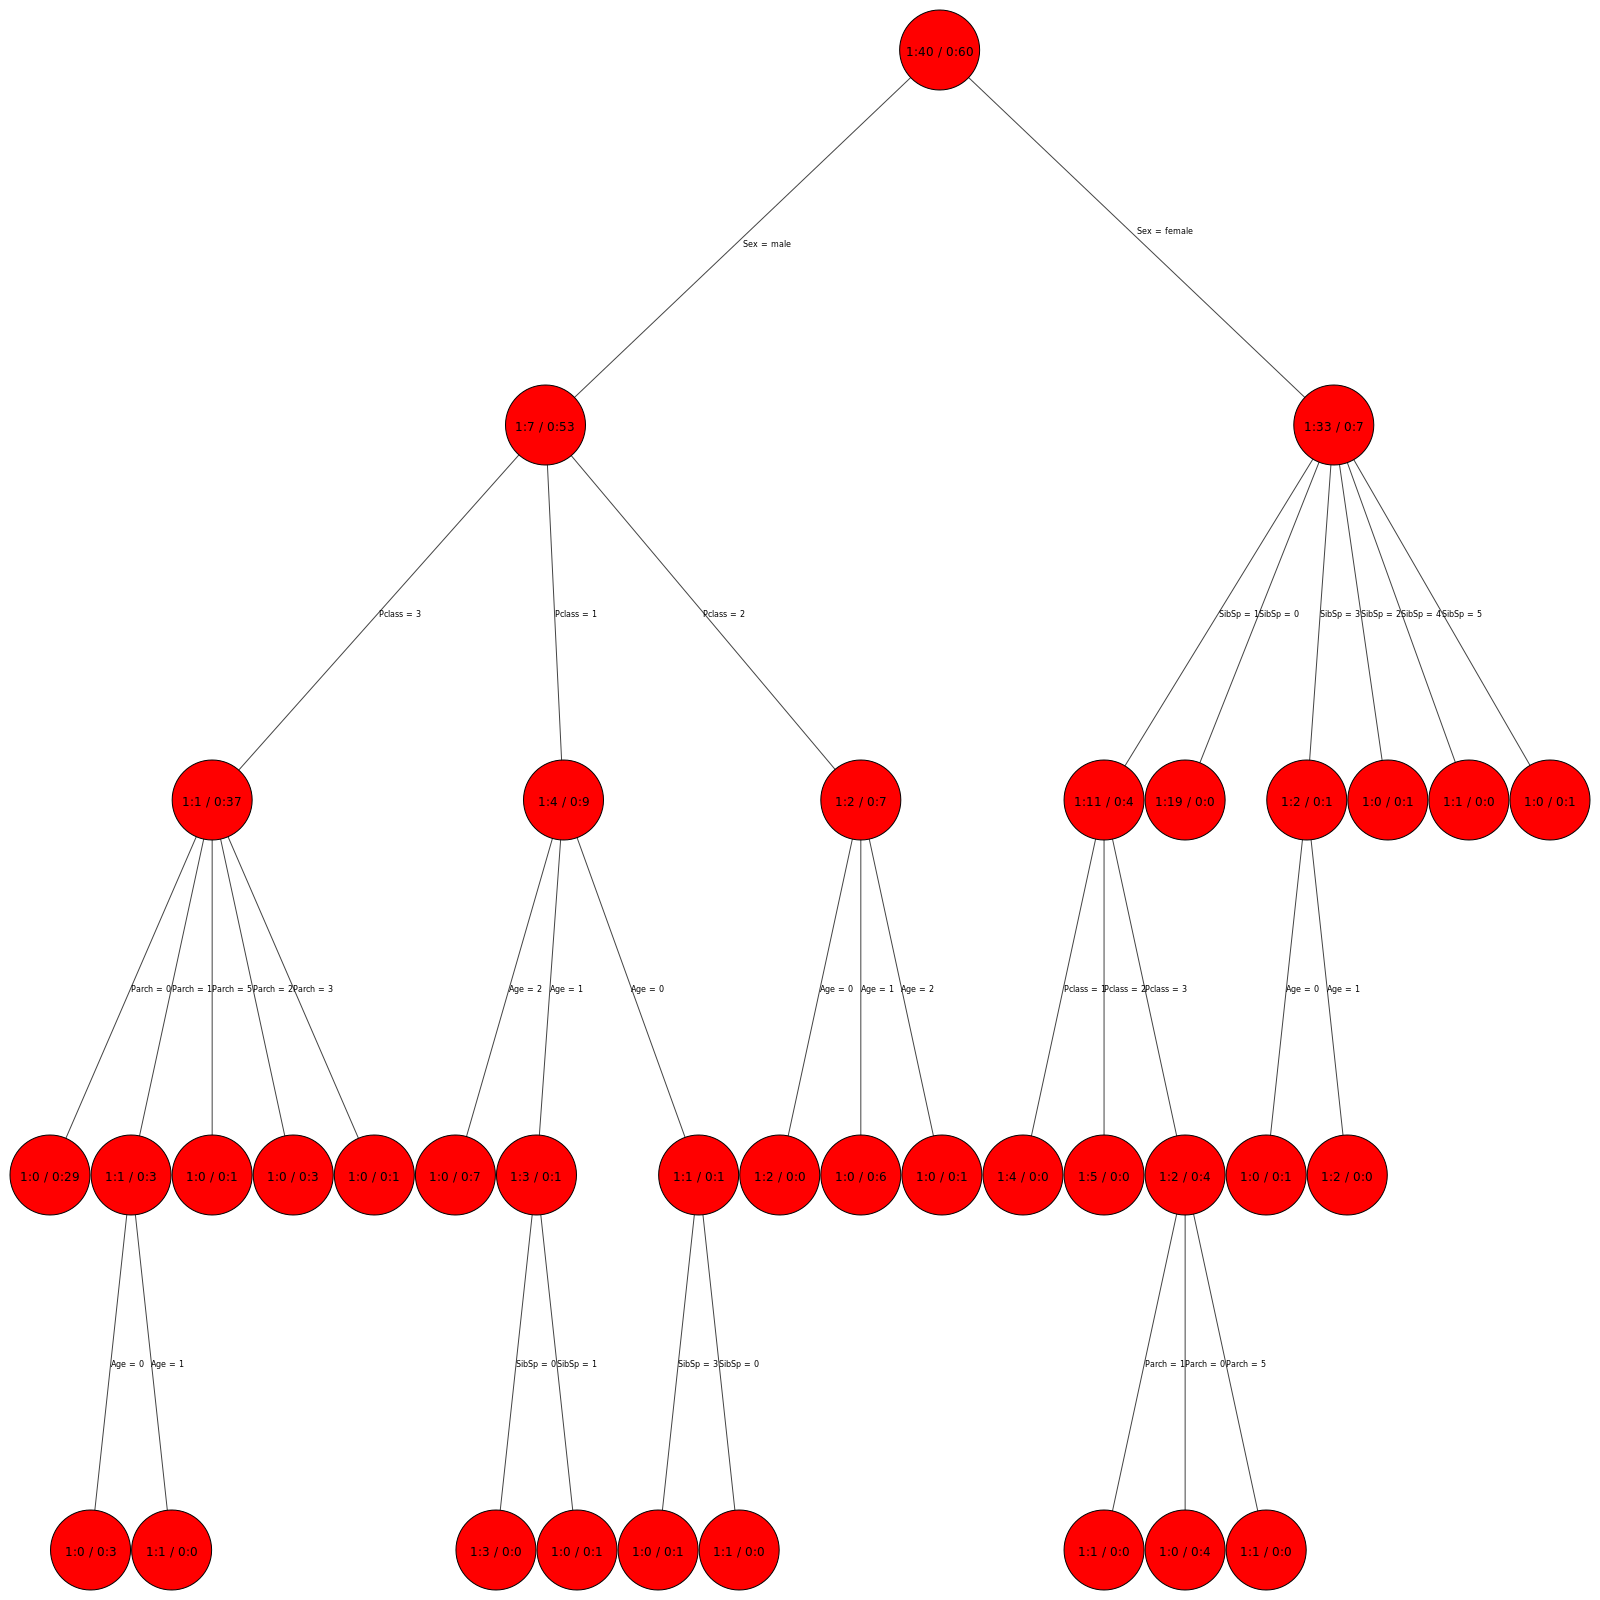
\includegraphics[width=\linewidth]{Dyskretny.png}
	\end{subfigure}
	\label{fig:dyskretne}
	\caption{Age jest atrybutem dyskretnym}
\end{figure}


\clearpage
\begin{figure}[h!]
	\subsection{Ciągły Age}
	\centering
	\begin{subfigure}[b]{1\linewidth}
		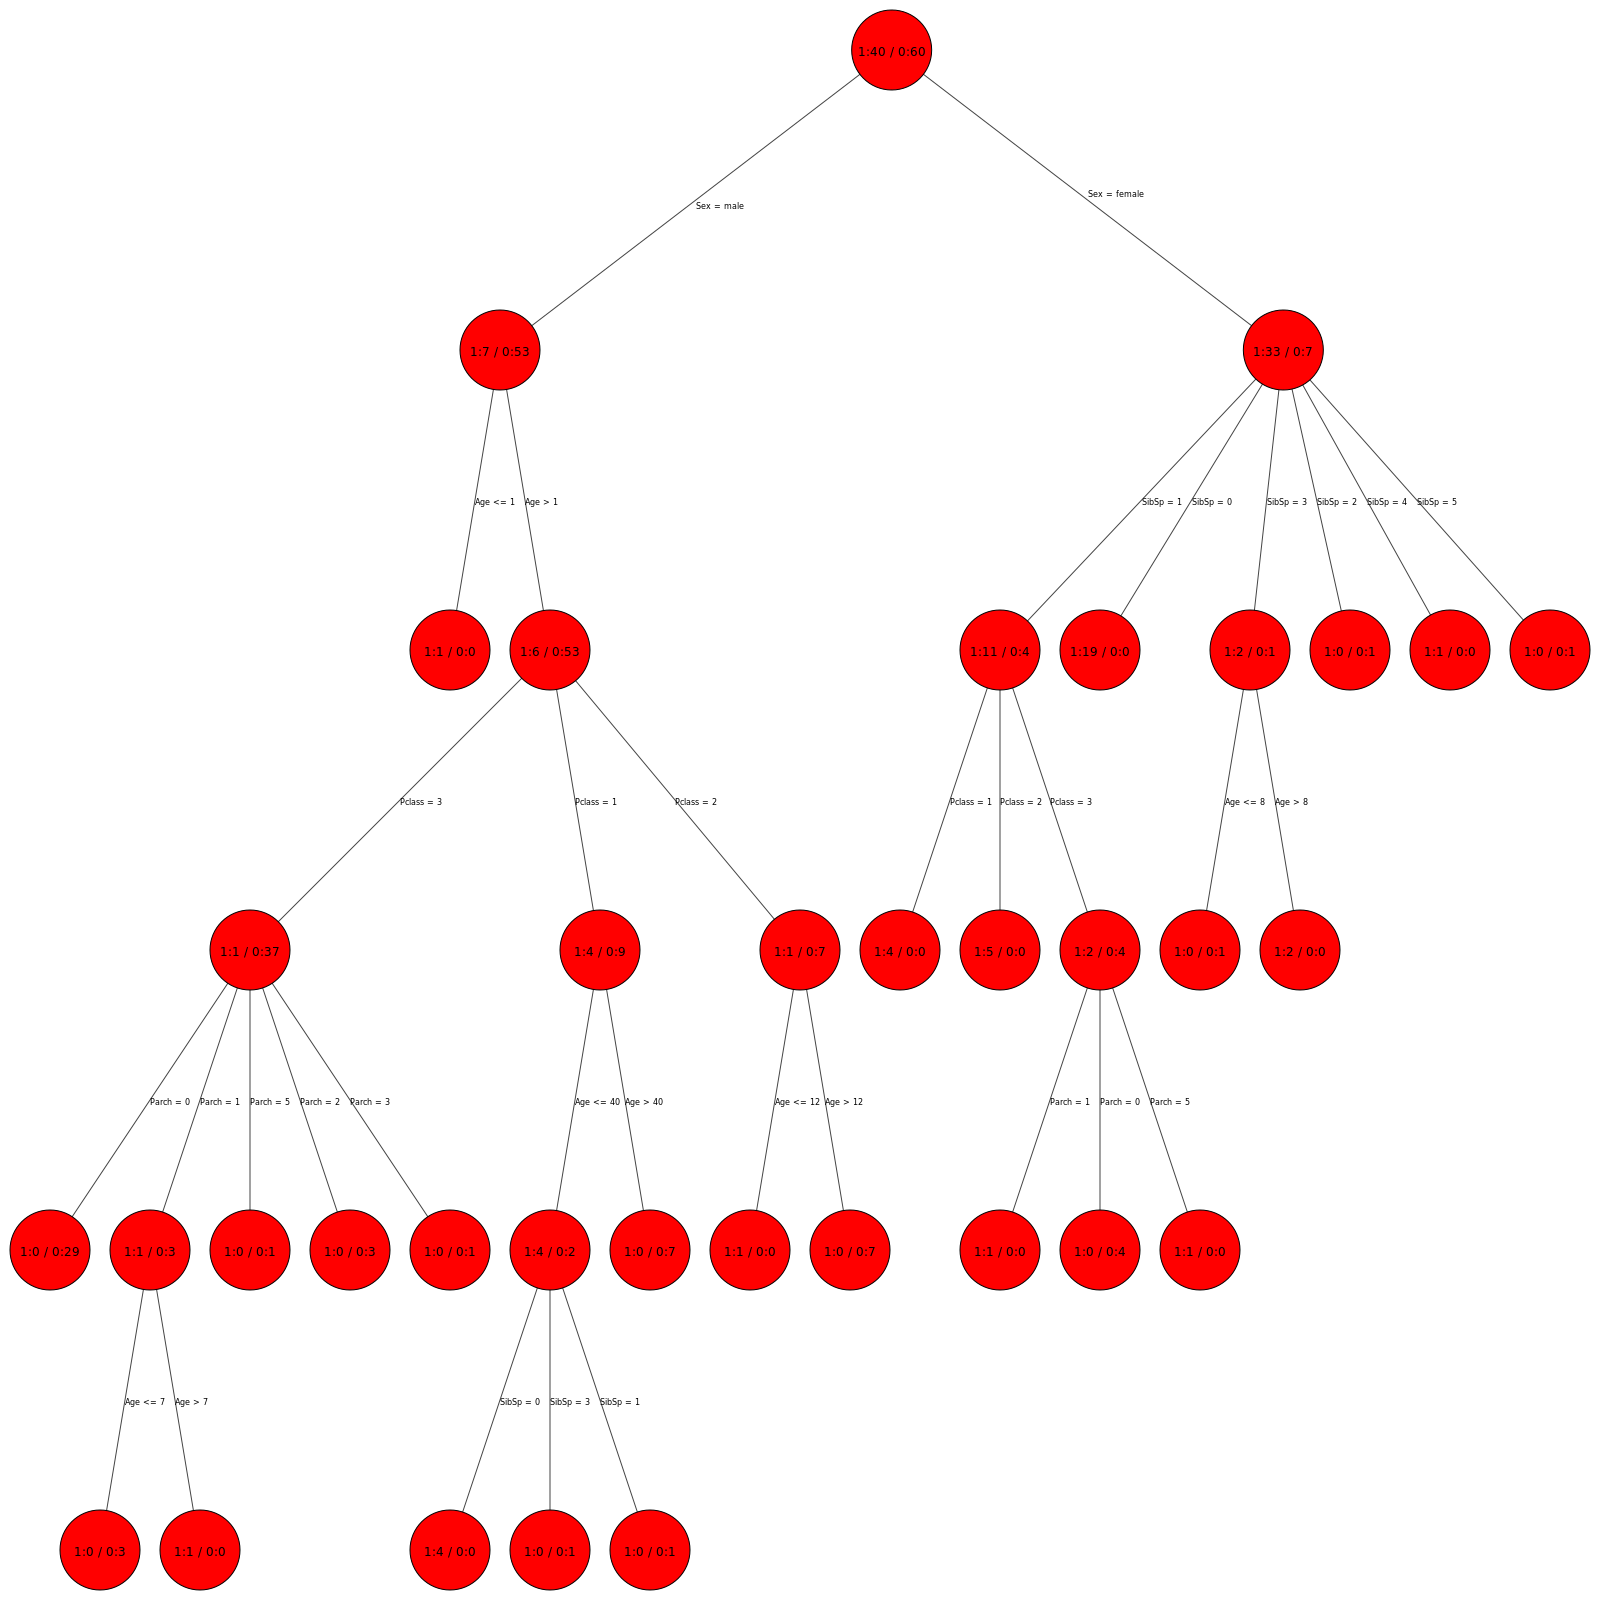
\includegraphics[width=\linewidth]{Ciagly.png}
	\end{subfigure}
	\label{fig:ciagle}
	\caption{Age jest atrybutem ciągłym}
\end{figure}

\end{document}
